\documentclass{beamer}

\usepackage{xltxtra}
\usepackage[lithuanian]{babel}
\usepackage{mathtools}
\usepackage{cite}
\usepackage{multimedia}
\usepackage{subfig}

\usepackage{hyperref}

\title{Difuzijos įtakos krūvininkų pernašai ir rekombinacijai skaičiavimas}

\author
{V. Valentinavičius}

\date{Vilnius, 2012}
\subject{Kursinis darbas}

\begin{document}
\frame{\titlepage}
  \begin{frame}
    \frametitle{Darbo tikslai}
    \begin{itemize}
      \item Naudojant skaitmeninį modeliavimą nustatyti eksperimentines sąlygas, kurioms esant negalima atmesti difuzijos įtakos rezultatams gautiems naudojant fotogeneruotų krūvininkų ištraukimo tiesiškai kylančia įtampa (photo-CELIV) metodiką.
	\item Naudojant skaitmeninį modeliavimą pademonstruoti ir paaiškinti difuzijos įtaką rekombinacijos koeficiento matavimams.
	\item Naudojant skaitmeninį modeliavimą patikrinti krūvininkų judrio skaičiavimų rezultatų validumą.
    \end{itemize}
  \end{frame}
  
  
  \begin{frame}
    \frametitle{Photo-CELIV}
    \begin{figure}
    	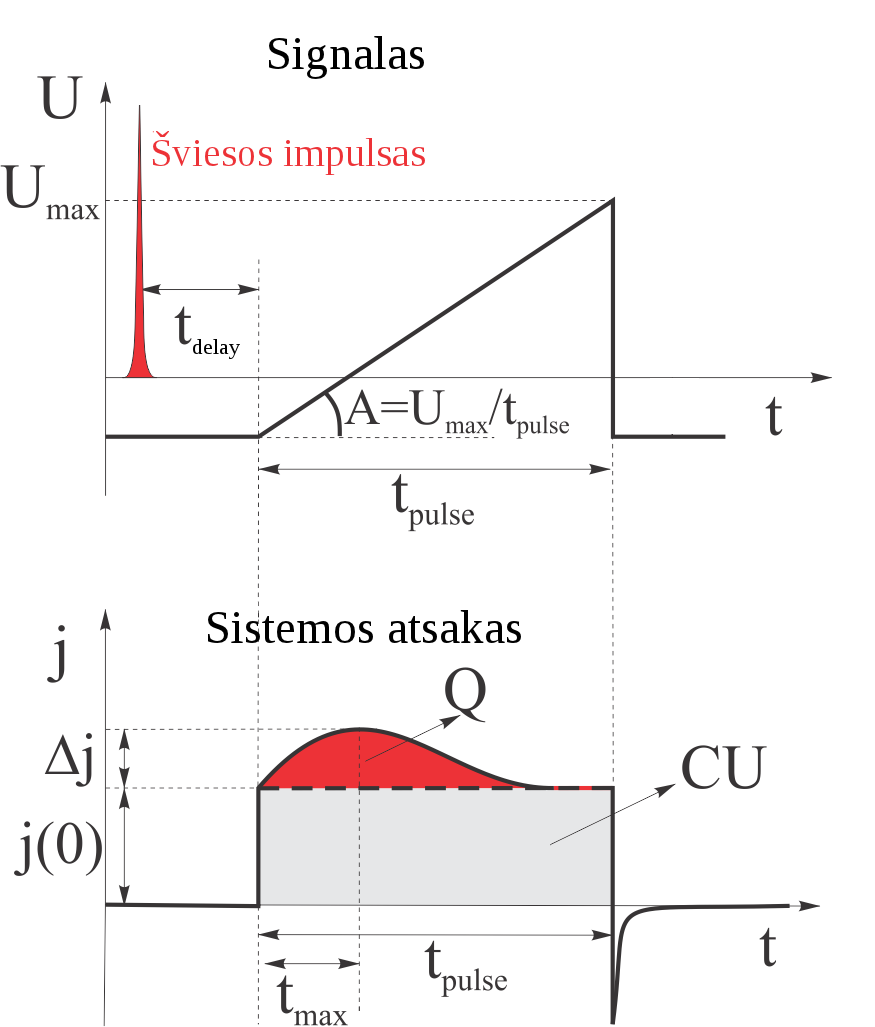
\includegraphics[height=0.8\textheight]{./media/celivTransients.png}
    \end{figure}
  \end{frame}
  
  \begin{frame}
	\frametitle{Photo-CELIV}
  \begin{columns}
    \begin{column}{.45\textwidth}
     \begin{block}{}
	\begin{itemize}
      \item $t_{max}$ proporcingas krūvininkų judriui
      \item $j_{max}$ priklauso nuo rekombinacijos
    \end{itemize}
    \end{block}
    \end{column}
    \begin{column}{.55\textwidth}
    \begin{block}{}
    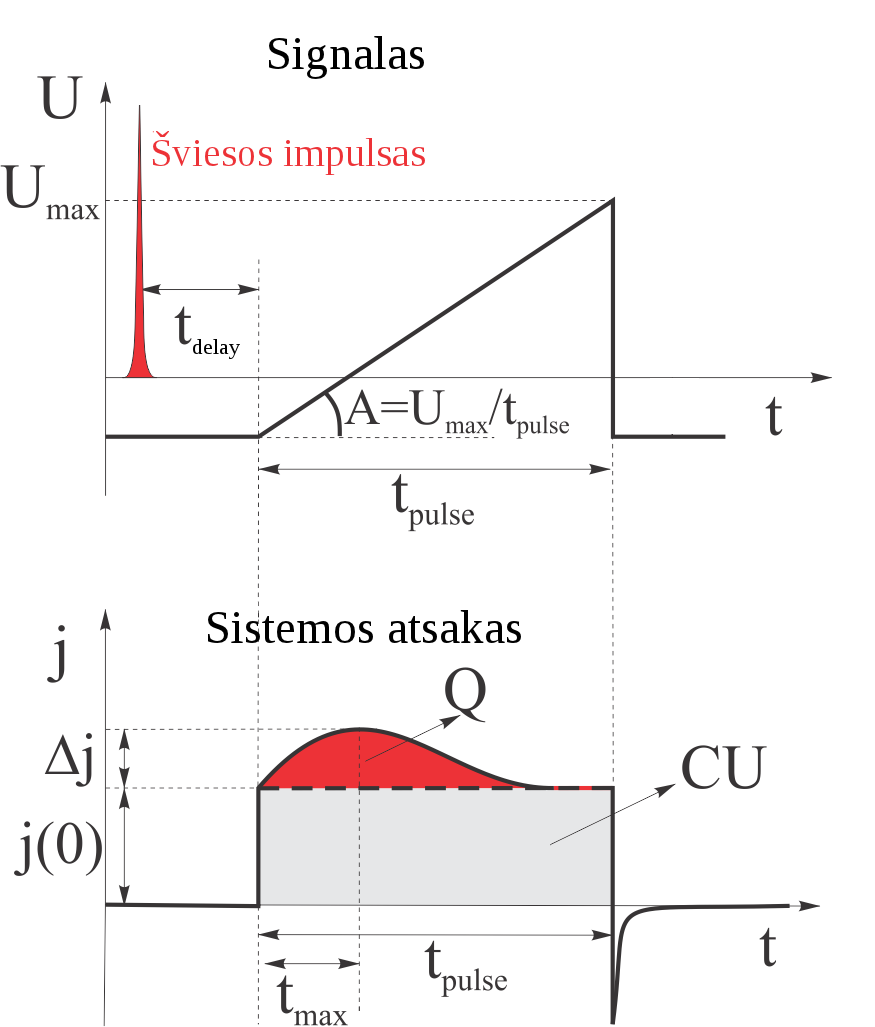
\includegraphics[height=0.8\textheight]{./media/celivTransients.png}
    \end{block}
    \end{column}
  \end{columns}
\end{frame}
  
  \begin{frame}
    \frametitle{Priemonės}
    \begin{itemize}
	\item Naudota autoriaus sukurta programa skirta spręsti krūvininkų pasiskirstymo uždavinius
	\item Programa leidžia atkartoti realaus eksperimento eigą ir sąlygas 
	\item Tirtas virtualaus bandinio elgesys simuliuojant photo-CELIV metodiką
	\end{itemize}    
	\begin{figure}
\centering
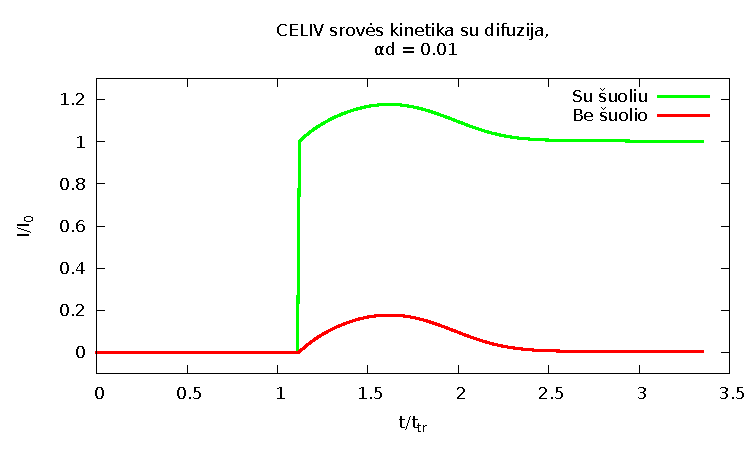
\includegraphics[height=0.5\textheight]{./media/pdf/jump.pdf} 
\end{figure}
  \end{frame}
  \begin{frame}
  	\frametitle{Analizuotos metodikos}
  	\begin{itemize}
  	\item Krūvininkų rekombinacijos įvertinimas pagal photo-CELIV kinetikų maksimumo soties vertę
  	\item Krūvininkų judrio skaičiavimas pagal photo-CELIV kinetikų maksimumo padėtį
  	\end{itemize}
  	\begin{figure}
    \centering
	\subfloat[$\alpha d = 0.1$]{
		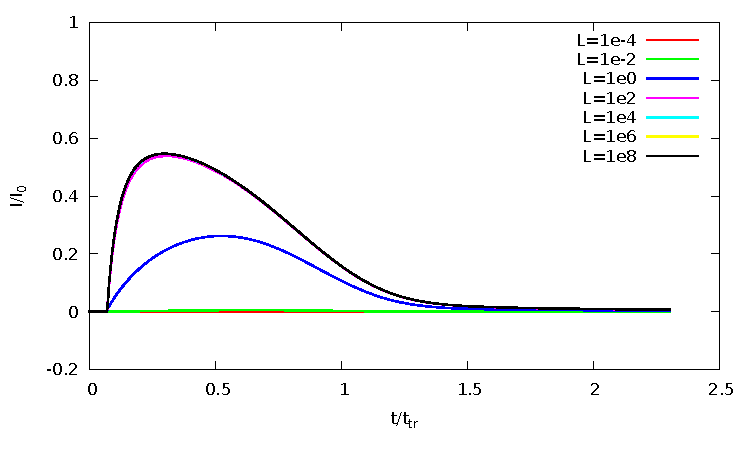
\includegraphics[width=0.5\textwidth]{./media/pdf/transient_ad01.pdf}
		}
	\subfloat[$\alpha d = 10$]{
		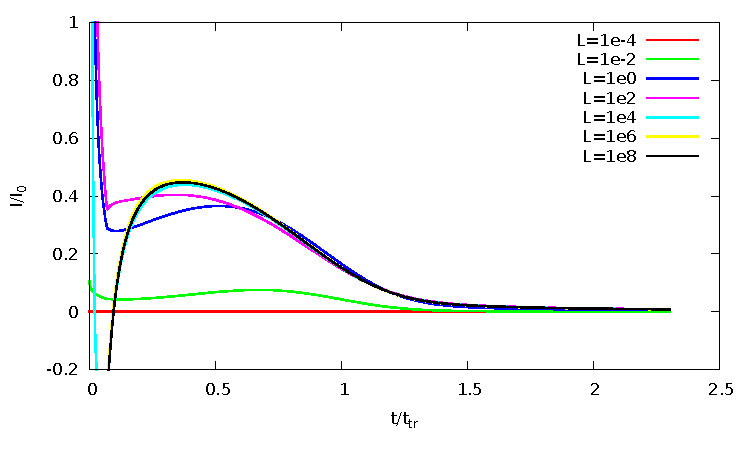
\includegraphics[width=0.5\textwidth]{./media/pdf/transient_ad10.pdf}
		}
\end{figure}
  \end{frame}
  
  
  \begin{frame}
    \frametitle{Parametrai}
    \begin{itemize}
	\item Krūvininkų judrių santykis \(\frac{\mu_n}{\mu_p} = 1000\)
	\item Bimolekulinė rekombinacija pagal Lanževeną \(B_L=\frac{e}{\varepsilon \varepsilon_0}(\mu_n+\mu_p)\)
	\item Difuzijos koeficientas suskaičiuojamas pagal Einšteino sąryšį \(D=\frac{k_B T \mu }{e}\)
	\item Šviesos sugertis skaičiuota pagal Beer-Lambert’o taisyklę, \(I(x)=I_0 e^{-\alpha x}\), kai kvantinis našumas lygus vienetui	
	\end{itemize}
  \end{frame}

  \begin{frame}
    \frametitle{Svarbiausi darbo rezultatai ir išvados}
    \framesubtitle{Difuzijos įtaka photo-CELIV srovės sotinimuisi}
    \begin{itemize}
		\item Difuzija padidina išmatuotą rekombinacijos koeficientą bandinyje, jei matavimui naudojama photo-CELIV srovės kinetikos soties vertė. Pokytis gali siekti 20-50\% priklausomai nuo krūvininkų sugerties profilio.
    \end{itemize}
  \end{frame}

  \begin{frame}
    \frametitle{Svarbiausi darbo rezultatai ir išvados}
    \framesubtitle{Difuzijos įtaka photo-CELIV srovės sotinimuisi}
    \begin{figure}
    	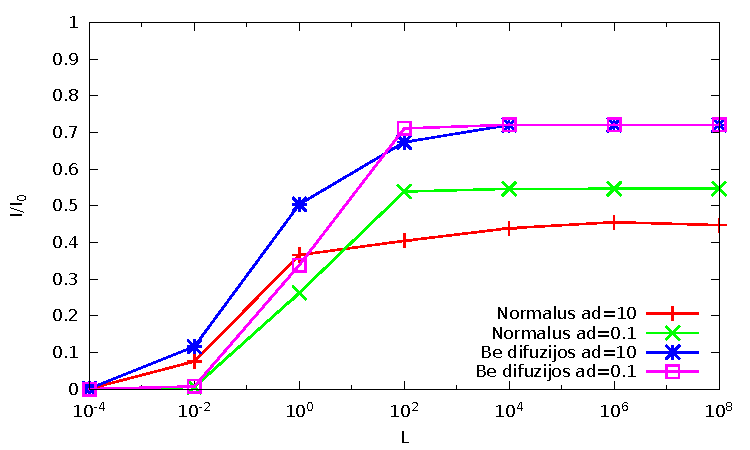
\includegraphics[width=0.9\textwidth]{./media/pdf/semilogsaturation.pdf}
    \end{figure}
    \begin{itemize}
    \item Photo-CELIV srovės kinetikos maksimumo vertės sotinimasis nuo šviesos intensyvumo parametro
    \end{itemize}
  \end{frame}
  
  \begin{frame}
    \frametitle{Svarbiausi darbo rezultatai ir išvados}
    \framesubtitle{Difuzijos įtaka judrio vertės skaičiavimui}
    \begin{itemize}
      \item Krūvininkų judrio matavimo rezultatai iš photo-CELIV kinetikos maksimumo padėties priklauso nuo užlaikymo trukmės. Tai lemia pradinio krūvininkų kiekio kitimas dėl rekombinacijos.
      \item Įskaičius difuziją, esant $t_{delay} < t_{tr}$ judrio vertė papildomai pakinta iki 2 kartų, priklausomai nuo pradinio pasiskirstymo. Difuzija pakeičia krūvininkų pasiskirstymo pavidalą.
    \end{itemize}
  \end{frame}
    
  \begin{frame}
    \frametitle{Svarbiausi darbo rezultatai ir išvados}
    \framesubtitle{Difuzijos įtaka judrio vertės skaičiavimui}
    \begin{figure}
    	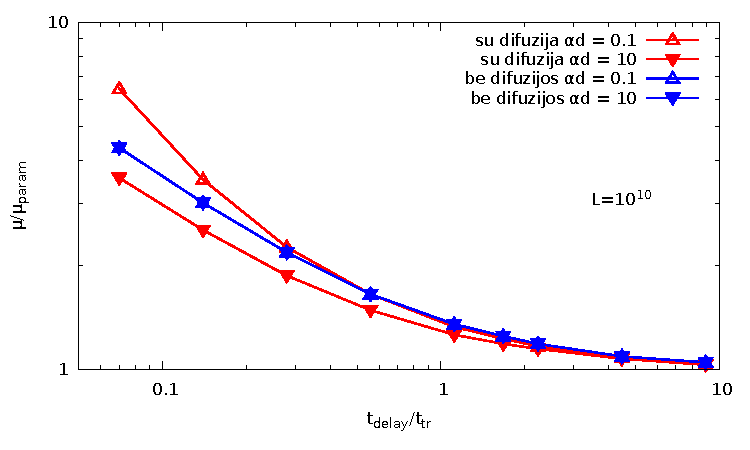
\includegraphics[width=0.9\textwidth]{./media/pdf/log_mobility.pdf}
    \end{figure}
    \begin{itemize}
    \item Pagal photo-CELIV srovės kinetikų maksimumo padėtis suskaičiuoto judrio priklausomybė nuo simuliacijos parametrų
    \end{itemize}
  \end{frame}
  
  \begin{frame}
  \frametitle{Pabaiga}
  Gal turite klausimų?
  \end{frame}
  
  \begin{frame}
  \frametitle{Priedai}
  \begin{equation}
  \frac{\partial n}{\partial t} = -\mu n \frac{e}{\varepsilon \varepsilon_0 S} \int_{0}^{x} x(n-p)dx -D \frac{\partial^2 n}{\partial x^2} -\eta B_L n p
  \end{equation}
  \end{frame}
  
  \begin{frame}
  \frametitle{Priedai}
  \begin{figure}
  \centering
    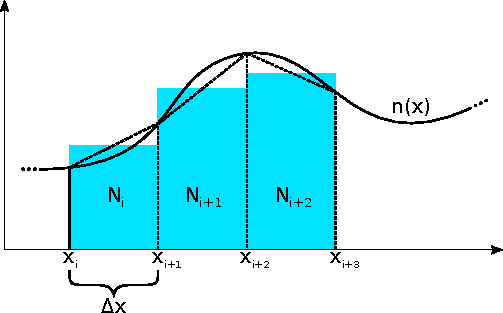
\includegraphics[scale=0.9]{./media/pdf/il1}
  \caption{Tankio diskretizavimas}
  \end{figure}
  \end{frame}
  
  \begin{frame}
  \frametitle{Priedai}
  \begin{figure}
  \centering
	\subfloat[Be užlaikymo]{
		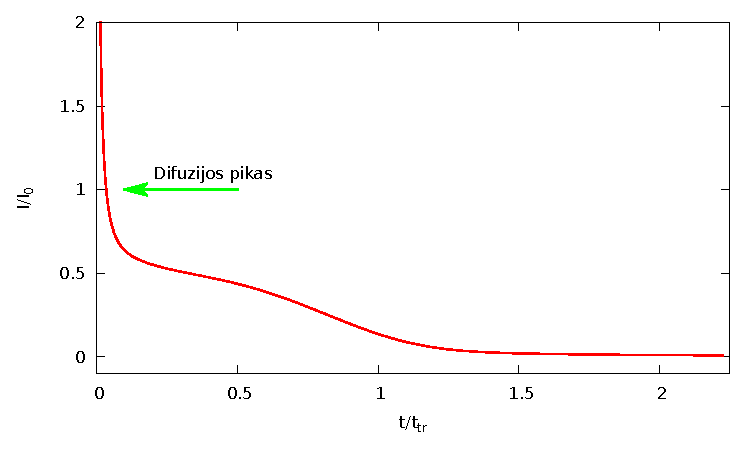
\includegraphics[width=0.5\textwidth]{./media/pdf/disappear.pdf}
		}
	\subfloat[Su užlaikymu]{
		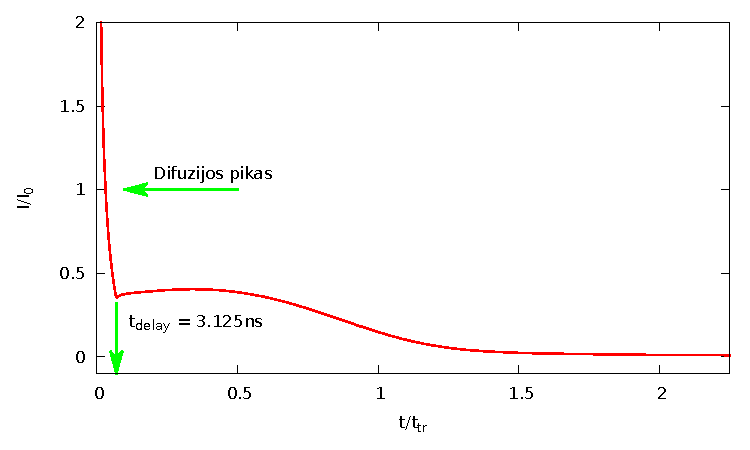
\includegraphics[width=0.5\textwidth]{./media/pdf/exist.pdf}
		}
  \caption{Difuzijos pikas paslepia photo-CELIV srovės kinetikos maksimumą, esant paviršiniam sužadinimui. Įvedus užlaikymo trukmę $t_{delay}$ galima išskirti srovės kinetikos maksimumą}

	\end{figure}
  \end{frame}
  
  \begin{frame}
  \frametitle{Priedai}
  \begin{figure}
  \centering
    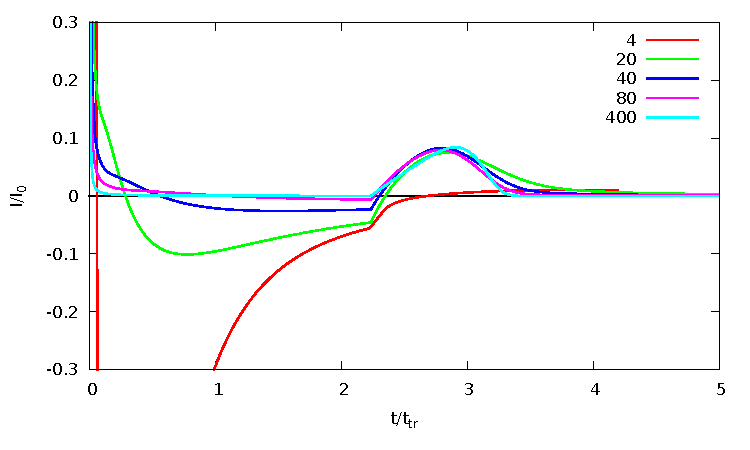
\includegraphics[width=0.9\textwidth]{./media/pdf/diff_drift.pdf}
  \caption{Photo-CELIV kinetikos su skirtingais $eU/kT$ esant paviršinei krūvininkų generacijai $\alpha d = 100$}
\end{figure}
  \end{frame}

\begin{frame}
\frametitle{Priedai}
\begin{figure}
    \centering
	\subfloat[$\alpha d = 0.1$]{
		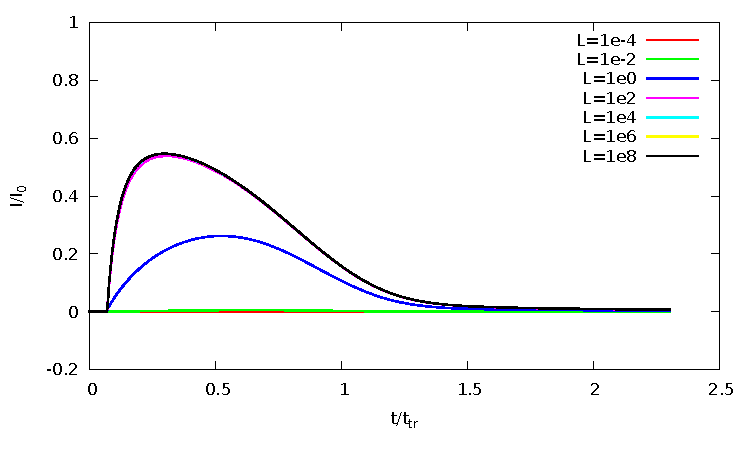
\includegraphics[width=0.5\textwidth]{./media/pdf/transient_ad01.pdf}
		}
	\subfloat[$\alpha d = 10$]{
		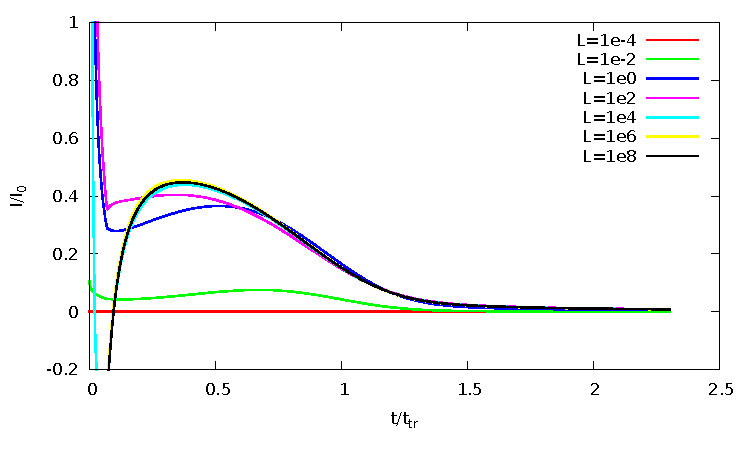
\includegraphics[width=0.5\textwidth]{./media/pdf/transient_ad10.pdf}
		}
  \caption{Photo-CELIV kinetikų pavidalo priklausomybė nuo šviesos intensyvumo, priklausomai nuo sugerties profilio, esant minimaliai užlaikymo trukmei $t_{delay} = 0.07t_{tr}$ ir įskaičius difuziją}
\end{figure}
\end{frame}

\begin{frame}
\frametitle{Priedai}
\begin{figure}
  \centering
    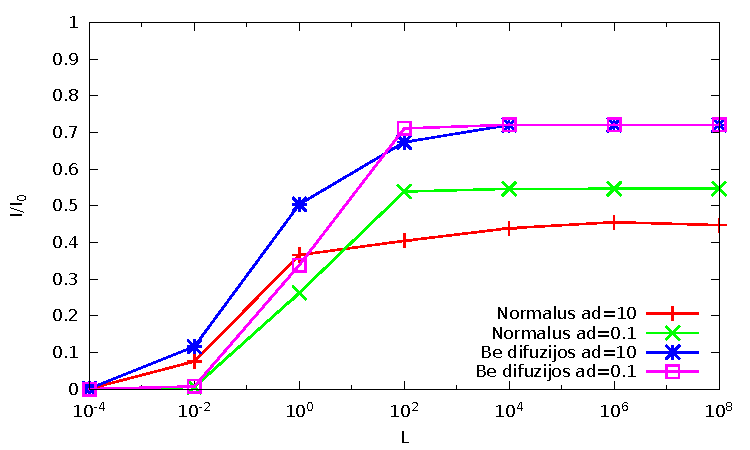
\includegraphics[width=0.9\textwidth]{./media/pdf/semilogsaturation.pdf}
  \caption{Photo-CELIV kinetikų maksimumo srovės vertės sotinimasis nuo šviesos intensyvumo, priklausomai nuo difuzijos ir sugerties profilio, esant minimaliai užlaikymo trukmei $t_{delay} = 0.07t_{tr}$}
\end{figure}
\end{frame}

\begin{frame}
\frametitle{Priedai}
\begin{figure}
  \centering
	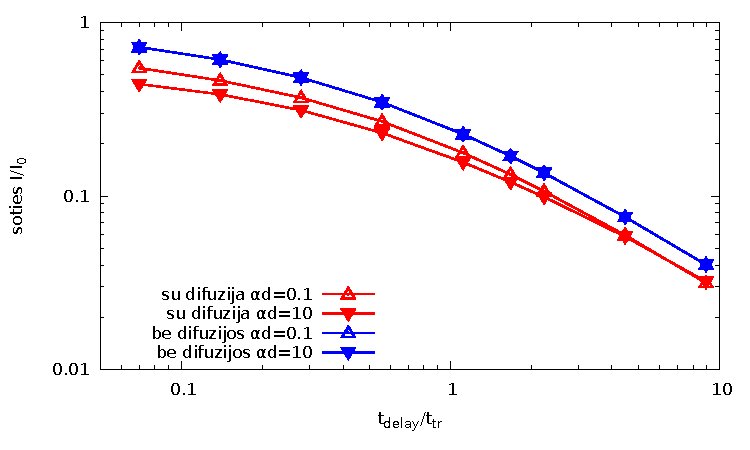
\includegraphics[width=0.9\textwidth]{./media/pdf/delays.pdf}
  \caption{Photo-CELIV srovės kinetikų soties vertės priklausomybės nuo užlaikymo trukmės $t_{delay}$}
\end{figure}
\end{frame}

\begin{frame}
\frametitle{Priedai}
\begin{figure}
  \centering
	\subfloat[$\alpha d = 0.1$]{
		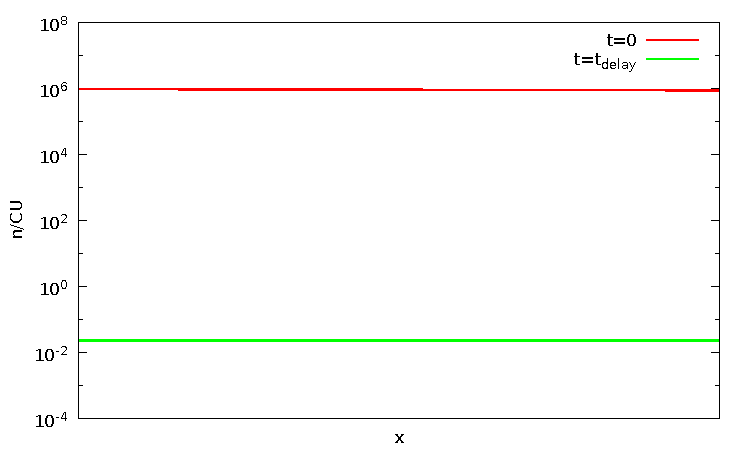
\includegraphics[width=0.5\textwidth]{./media/pdf/recomb_ad01.pdf}
		}
	\subfloat[$\alpha d = 10$]{
		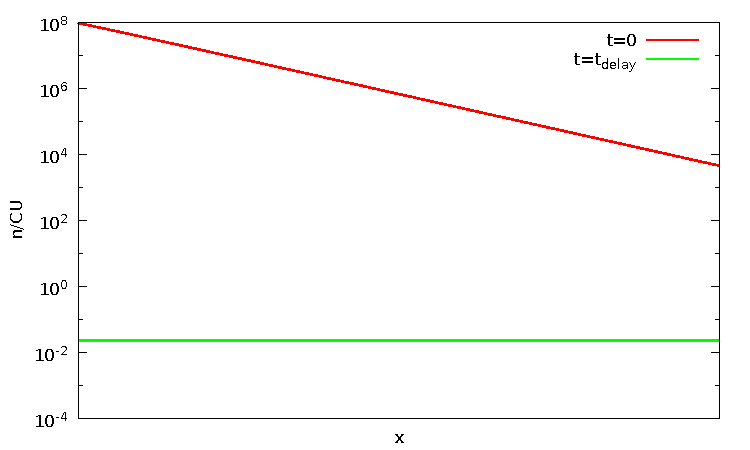
\includegraphics[width=0.5\textwidth]{./media/pdf/recomb_ad10.pdf}
		}
  \caption{Dėl rekombinacijos susilyginančios pradinės sąlygos per užlaikymo trukmę $t_{delay} = 0.07t_{tr}$, kai nėra difuzijos.}
\end{figure}
\end{frame}

\begin{frame}
\frametitle{Priedai}
\begin{figure}
  \centering
	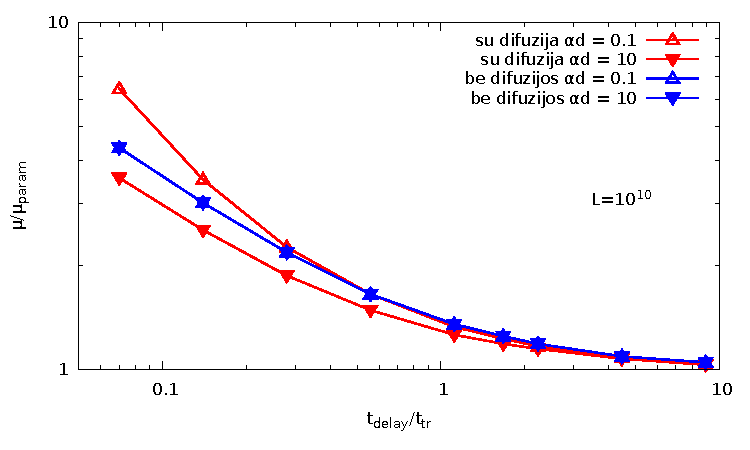
\includegraphics[width=0.9\textwidth]{./media/pdf/log_mobility.pdf}
  \caption{Krūvininkų judrio skaičiavimo pagal formulę $\mu = \frac{2d^2}{3At_{max}^2}$ rezultatų priklausomybė nuo $t_{delay}$}
\end{figure}
\end{frame}

\end{document}